\chapter{
Beyond SBDRL
 \draftnote{blue}{V0}{}
}

\whendraft{
\noindent\rule{\textwidth}{1mm}
\textbf{To do:}
\begin{enumerate}
    \item Local algebra
    \begin{enumerate}
        \item If $a \sim_{w} a'$ for all $w \in W$, then $a \sim a'$.
    \end{enumerate}
\end{enumerate}
\noindent\rule{\textwidth}{1mm}
}













%%%%%%%%%%%%%%%%%%%%%%%%%%%%%%%%%%%%%%%%%%%%%
\section{Local algebra algorithm}
\whendraft{
	\noindent\rule{\textwidth}{1mm}
	\textbf{To do:}
	\begin{enumerate}
		\item Proof that the algorithm halts.
            \item Proof that when the algorithm halts it contains the complete algebra.
            \item Put the full algorithm in the appendices.
	\end{enumerate}
	\noindent\rule{\textwidth}{1mm}
}

%%%%%%%%%%%%%%%%%%%%%%%%%%%%%%%%%%%%%%%%%%%%%
\subsection{Generating the equivalence classes}

To generate the local algebra, we altered algorithm \ref{alg:GenerateEquivClasses} to use a different $\Call{ComputeActionFunction}$ function.
Since our $\Call{LocalComputeActionFunction}$ requires an additional initial state parameter $w^{*}$, we must also feed that parameter into $\Call{GenerateEquivClasses}$ and $\Call{ProcessCandidate}$.
Other than those changes, the algorithm for generating the equivalence classes for the local algebra is the same as for the global algebra.

\begin{algorithm}[H]
	\caption{
		Compute the part of the action function $f_{a}: W \to W$ that sends $w^{*} \mapsto a \ast w^{*}$.
	}
	\hrulefill
	\begin{algorithmic}[1]
		\Procedure{LocalComputeActionFunction}{$a$, \; $\mathscr{W}$, \; $w^{*}$}
		\State $f_{a} \gets (\emptyset \to \emptyset)$
		\State $w_{a} \gets$ \Call{GenerateActionOutcome}{$a$, \; $w^{*}$, \; $\hat{\ast}$}
		\State $f_{a} \gets f_{a} \cup f_{a}'$ where $f_{a}': \{w^{*}\} \to \{w_{a}\}$ such that $f_{a}'(w^{*}) = w_{a}$
		\State \Return $f_{a}$
		\EndProcedure
	\end{algorithmic}
\end{algorithm}

%%%%%%%%%%%%%%%%%%%%%%%%%%%%%%%%%%%%%%%%%%%%%
\subsection{Generating the Cayley table}

To generate the local Cayley table, we use algorithm \ref{alg:GenerateCayley} with a different $\Call{ComputeCompositionActionFunction}$ function.

\begin{algorithm}[H]
	\caption{
		Compute the action function for the combination $l_{L} \circ l_{R}$ using \Call{LocalComputeActionFunction}.
	}
	\hrulefill
	\begin{algorithmic}[1]
		\Procedure{ComputeCompositionActionFunction}{$l_{L}$, \; $l_{R}$, \; $\mathcal{T}$, \; $\rho$, \; $\mathscr{W}$, \; $w^{*}$}
		      \State $a \gets \operatorname{Combine}(l_{L}, \; l_{R})$
                \State $f_{a} \gets$ \Call{LocalComputeActionFunction}{$a$, \; $\mathscr{W}$, \; $w^{*}$}
                \State \Return $f_{a}$
		\EndProcedure
	\end{algorithmic}
\end{algorithm}





%%%%%%%%%%%%%%%%%%%%%%%%%%%%%%%%%%%%%%%%%%
\chapter{(OLD) Beyond SBDRL (to be converted over)}
%%%%%%%%%%%%%%%%%%%%%%%%%%%%%%%%%%%%%%%%%%%%%%%%%%%%%%%%%%%%%%%%%%%%%%%%%%%%%
\section{Worlds without inverse actions}

In this section, we consider worlds that do not necessarily satisfy world condition ref[wldcon:inverse-actions] but do satisfy world condition ref[wldcon:unrestricted-actions].

\begin{proposition}\label{prp:wc1_gives_monoid_action}
    Consider a world $\mathscr{W}$ with a set $W$ of world states and containing an agent with a set $A$ of actions.
    If $\mathscr{W}$ satisfies world condition ref[wldcon:unrestricted-actions], then $*: (A/\sim) \times W \to W'$, where $W' \subseteq W$, is the action of a monoid $A/\sim$ on $W$.
\end{proposition}
\begin{proof}
    (1) Totality of $A/\sim$ is given by world condition ref[wldcon:unrestricted-actions].
    (2) Associativity of $A/\sim$ is given by proposition ref[prp:Asim-associative].
    (3) Identity element of $A/\sim$ is given by proposition ref[prp:Asim-identity].
    Since $A/\sim$ satisfies properties (1), (2), and (3), $A/\sim$ is a monoid.
    
    $*$ is defined for any $a \in A$ and $w \in W$, therefore $*$ is a monoid action.
\end{proof}

\begin{remark}
    If all actions are reversible in $\mathscr{W}$ then $W' = W$.
    If any action is irreversible in $\mathscr{W}$ then $W' \subset W$.
\end{remark}

%%%%%%%%%%%%%%%%%%%%%%%%%%%%%%%%%%%%%%%%%%%%%%%%%%%%%%%%%%%%%%%%%%%%%%%%%%%
\subsection{Example 1: reversible action-inhomogeneous world}\label{sec:identity reversible action-inhomogeneous world}

\paragraph{Properties and structure of $A/\sim$}
The action Cayley table for this world with the identity treatment of the walls contains 26 elements.
As shown in Table \ref{tab:identity-walls-properties}, $A/\sim$ is a monoid.

\begin{table}[H]
    \centering
    \begin{tabular}{c|c}
        \textbf{Property}   & \textbf{Present?} \\
        \hline
        Totality            & Y\\
        Identity            & Y\\
        Inverse             & N\\
        Associative         & Y\\
        Commutative         & Y
    \end{tabular}
    \caption{Properties of the $A/\sim$ algebra.}
    \label{tab:identity-walls-properties}
\end{table}


For $\mathscr{W}_{wall}$ with restricted actions treated as identity actions, every action is reversible from a particular state $w \in W$.
However, the action that takes $a$ back to its starting state is not necessarily the same any starting state $w \in W$.
For the inverse property to be present, the inverse for each element must be the same from any starting state (\textit{i.e.}, the inverse must be independent of the starting state).
$\mathscr{W}_{wall}$ with restricted actions treated as identity actions is proof that it is possible to have a world where all actions are reversible but for some of those actions to not have an inverse action.


%%%%%%%%%%%%%%%%%%%%%%%%%%%%%%%%%%%%%%%%%%
\subsection{Example 2: Reversible action-inhomogenous world without walls}

Consider a world $\mathscr{W}_{block}$ with the world states in Figure \ref{fig:movable_block_world_states} and with movement along a single 1D cyclical axis with a movable block.
If the agent is in the location directly to the left of the block and moves into the block, the block moves one location in the direction of the agent's movement and the agent moves into the location previously occupied by the block (see Table \ref{tab:4x1-gridworld-minimum-transitions-moveable-block} and Figure \ref{fig:4x1-block-min-actions-wall}).

\begin{figure}[htbp]
  \centering
  \begin{subfigure}{0.48\textwidth}
    \centering
    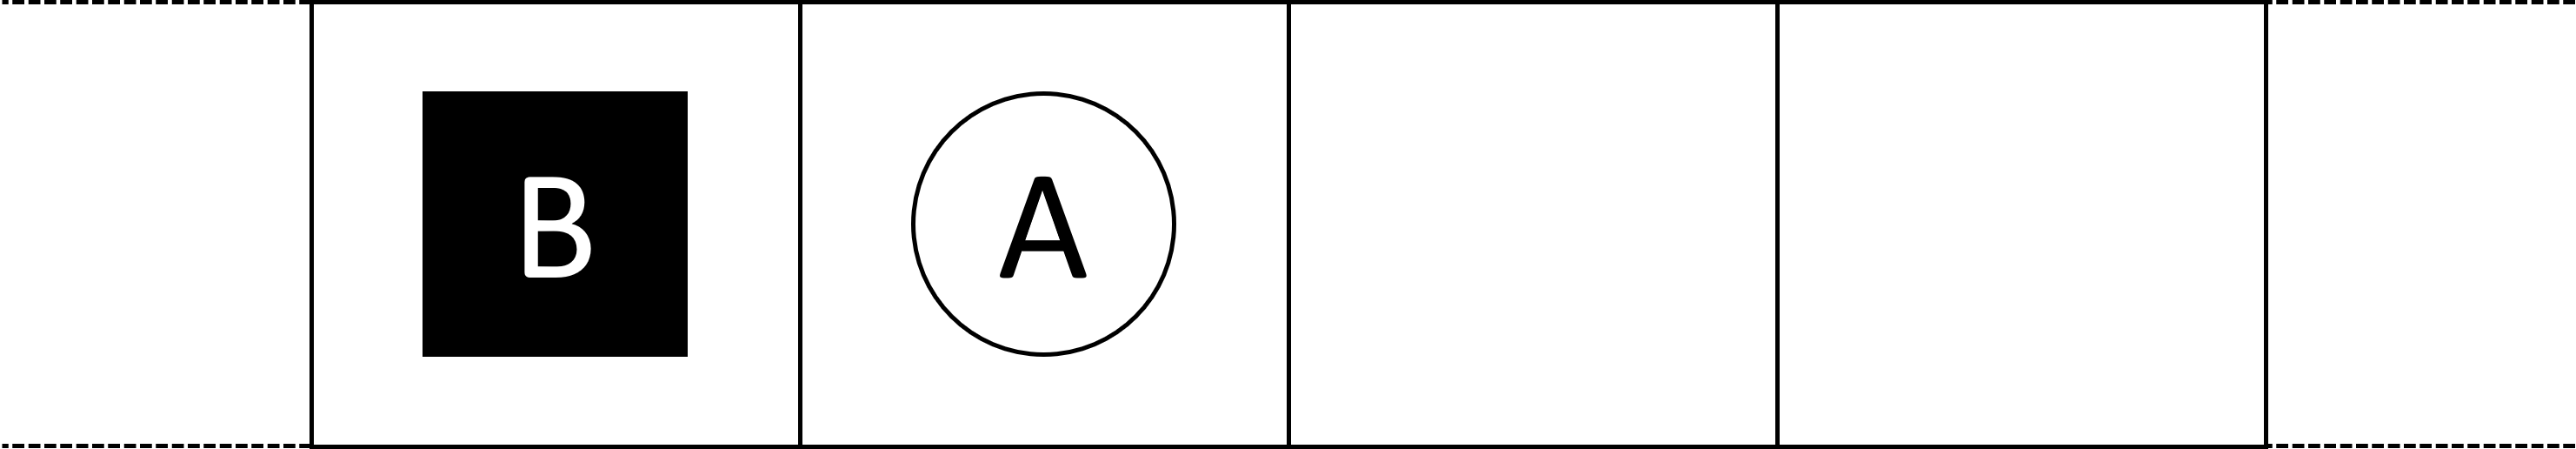
\includegraphics[width=\textwidth]{5BeyondSBDRL/Old/Images/Movable_block_world_states/w0.png}
    \caption{$w_{0}$}
  \end{subfigure}%
  \hfill
  \begin{subfigure}{0.48\textwidth}
    \centering
    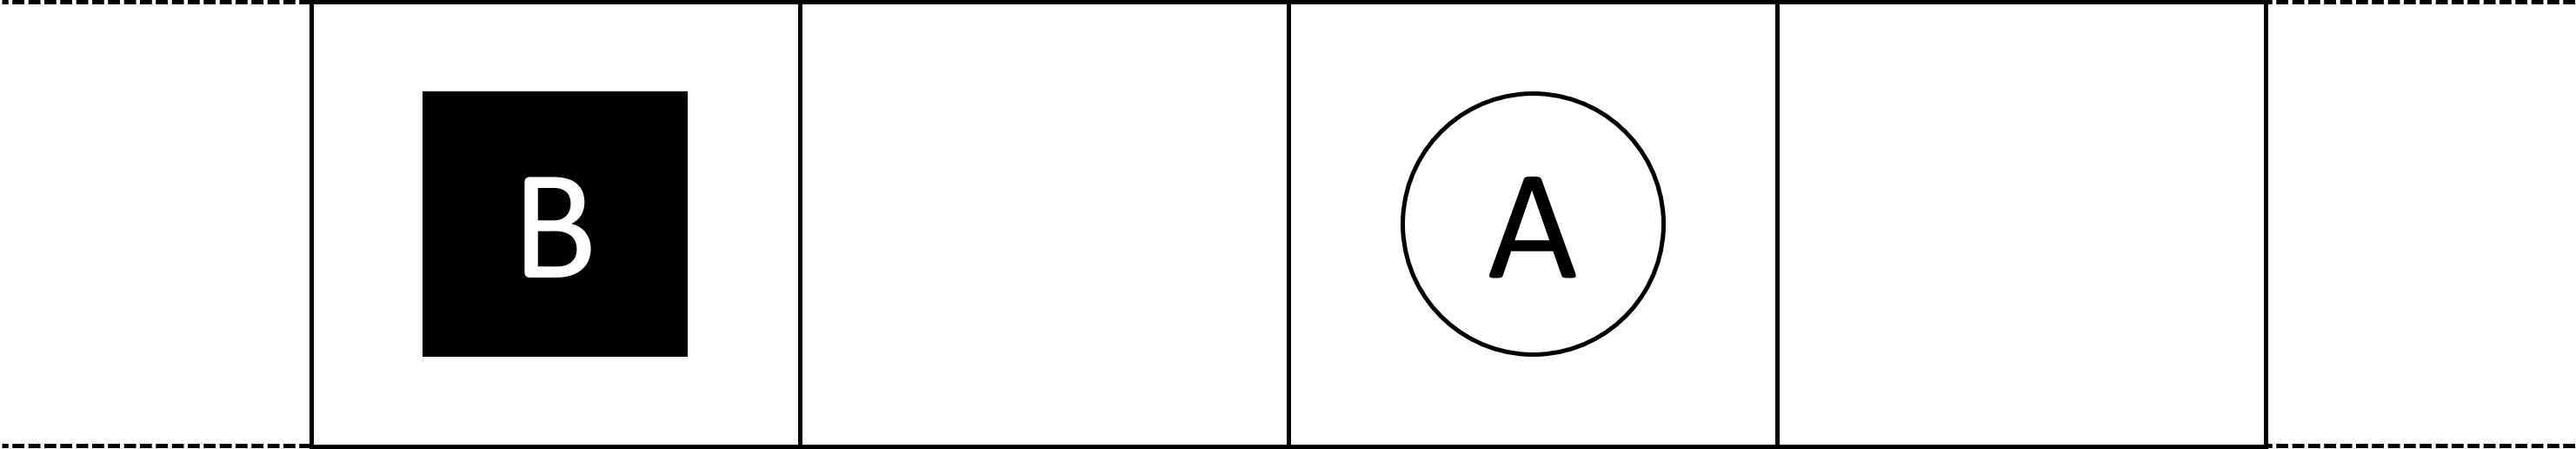
\includegraphics[width=\textwidth]{5BeyondSBDRL/Old/Images/Movable_block_world_states/w1.png}
    \caption{$w_{1}$}
  \end{subfigure}%
  \vspace{0.5cm}
  \begin{subfigure}{0.48\textwidth}
    \centering
    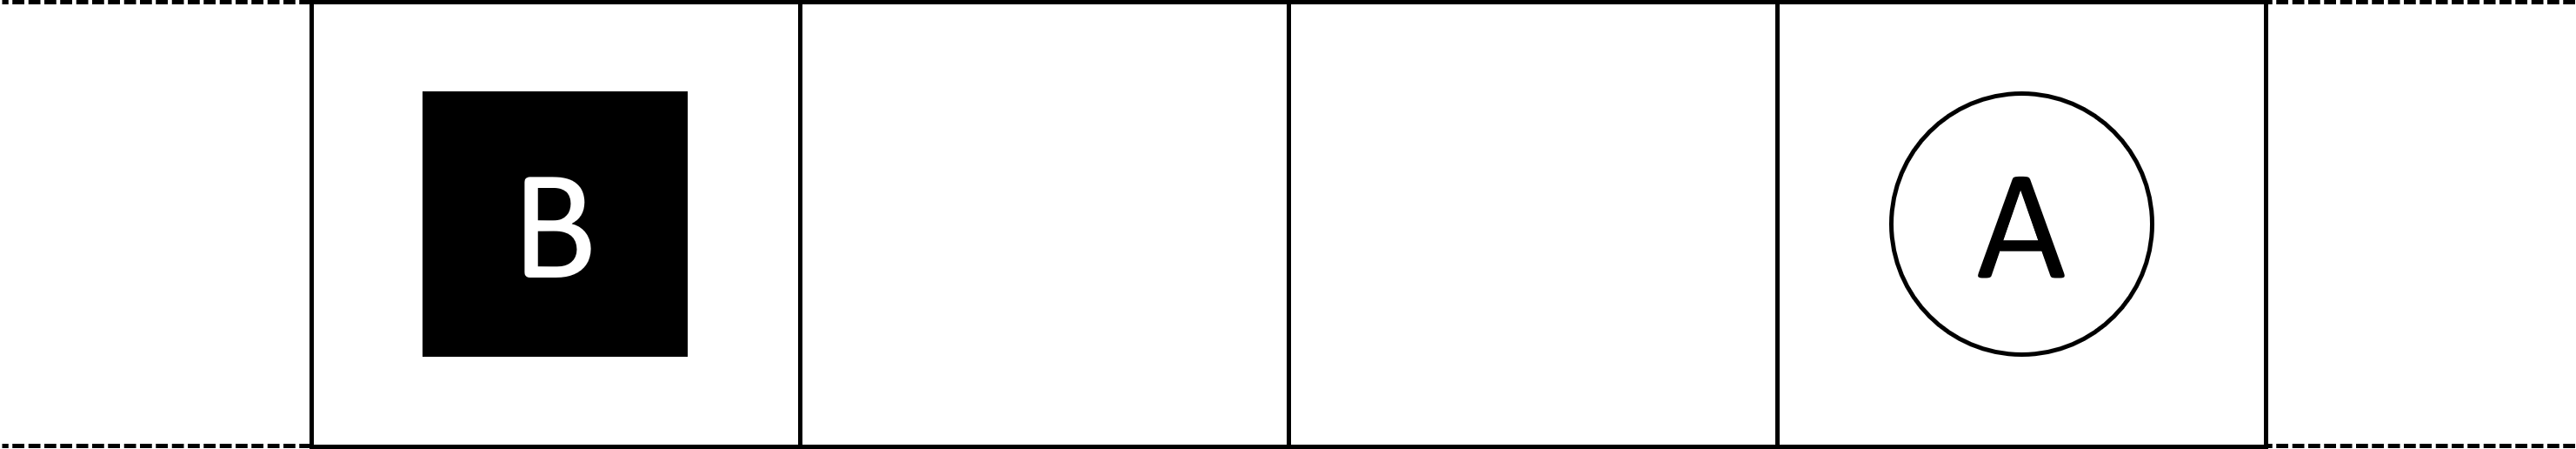
\includegraphics[width=\textwidth]{5BeyondSBDRL/Old/Images/Movable_block_world_states/w2.png}
    \caption{$w_{2}$}
  \end{subfigure}%
  \hfill
  \begin{subfigure}{0.48\textwidth}
    \centering
    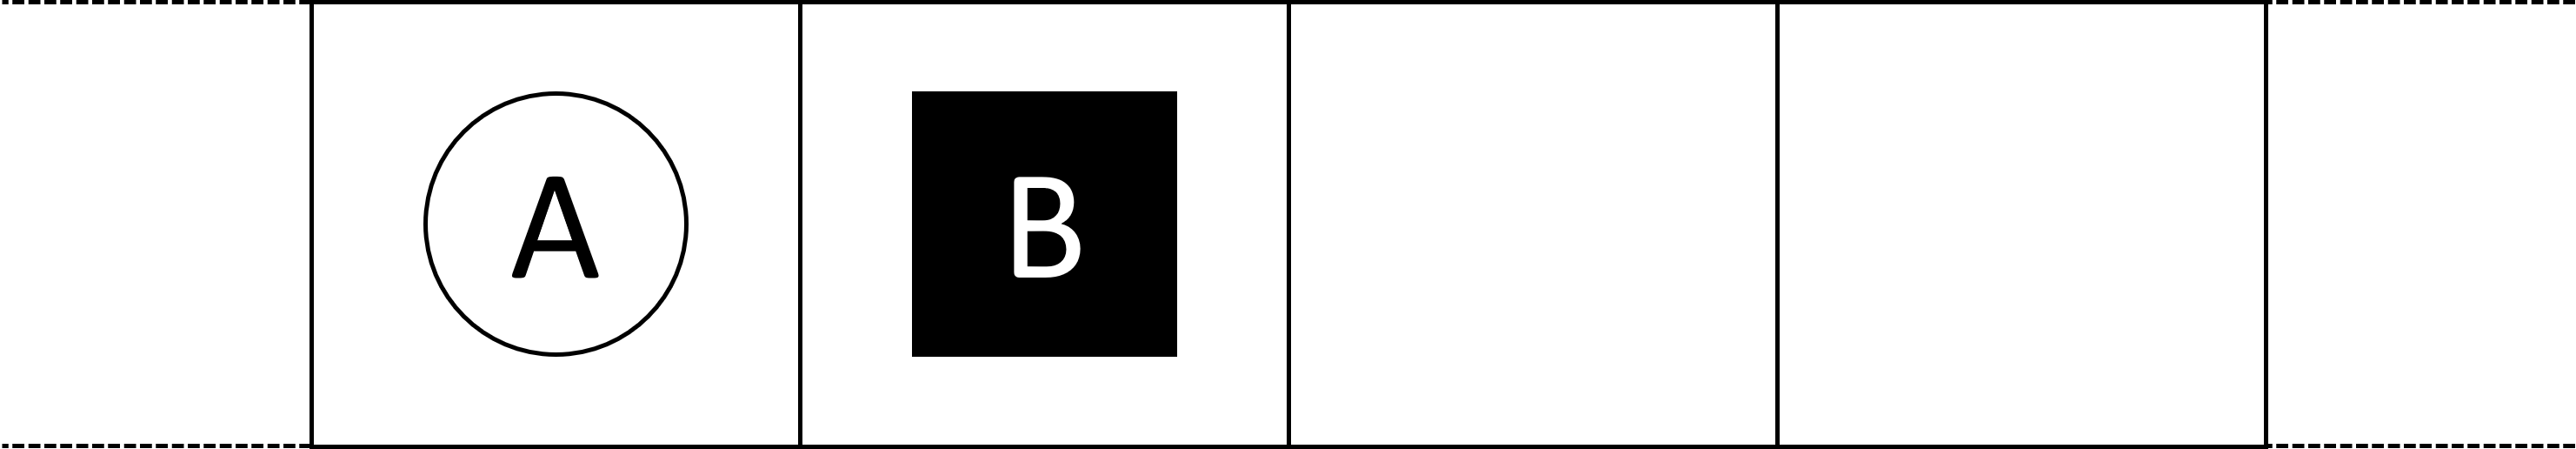
\includegraphics[width=\textwidth]{5BeyondSBDRL/Old/Images/Movable_block_world_states/w3.png}
    \caption{$w_{3}$}
  \end{subfigure}%
  \vspace{0.5cm}
  \begin{subfigure}{0.48\textwidth}
    \centering
    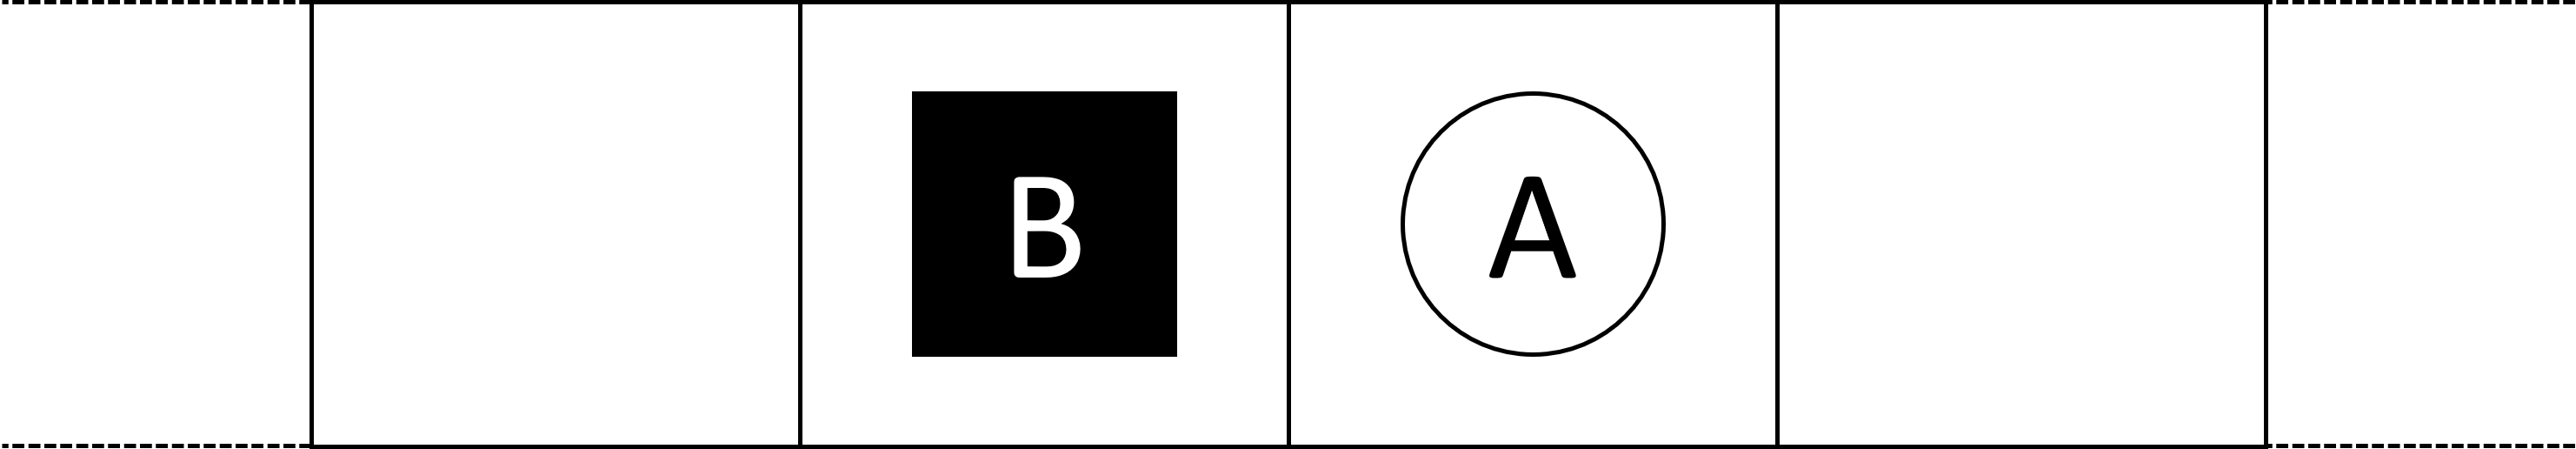
\includegraphics[width=\textwidth]{5BeyondSBDRL/Old/Images/Movable_block_world_states/w4.png}
    \caption{$w_{4}$}
  \end{subfigure}%
  \hfill
  \begin{subfigure}{0.48\textwidth}
    \centering
    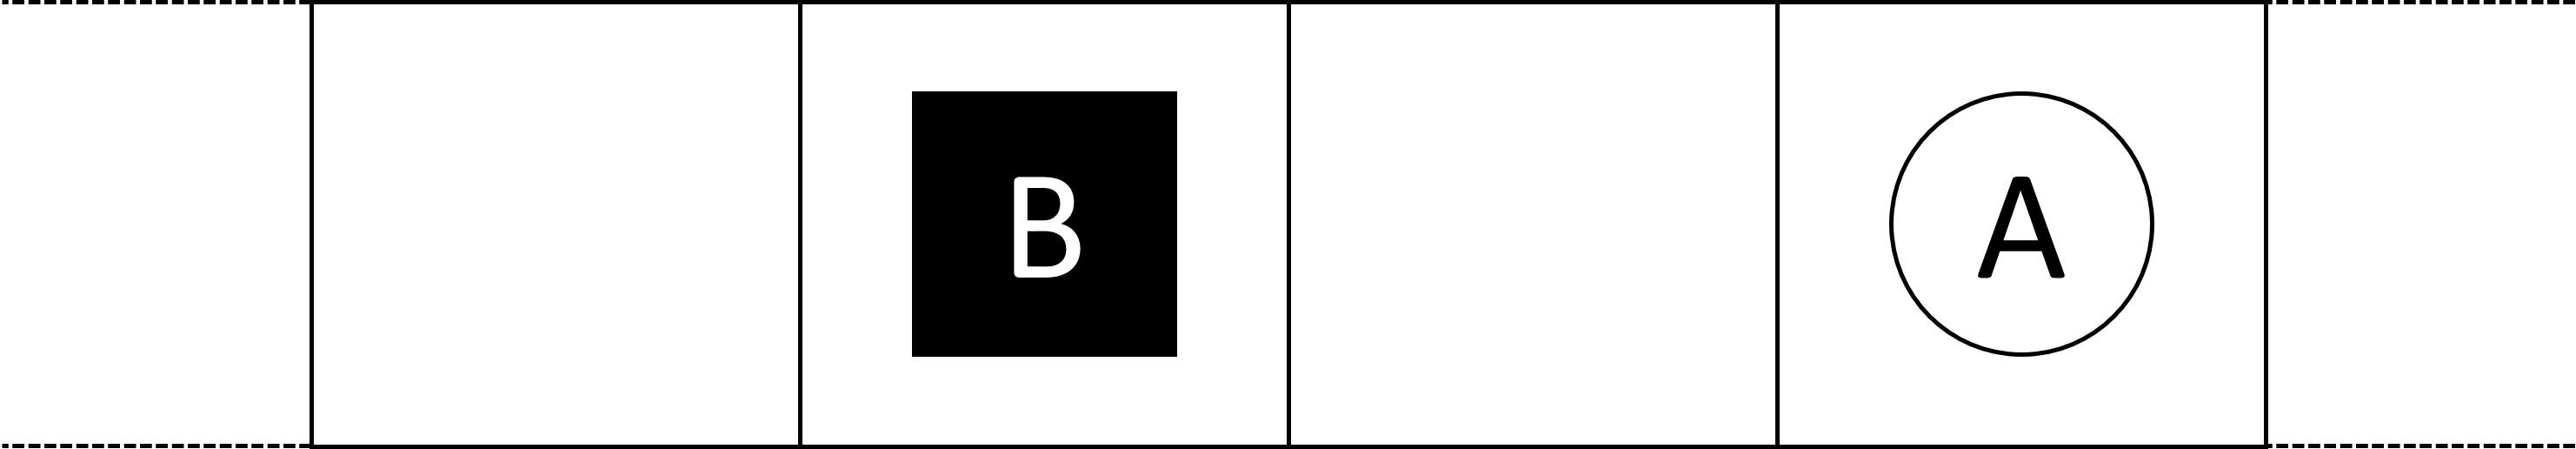
\includegraphics[width=\textwidth]{5BeyondSBDRL/Old/Images/Movable_block_world_states/w5.png}
    \caption{$w_{5}$}
  \end{subfigure}%
  \vspace{0.5cm}
  \begin{subfigure}{0.48\textwidth}
    \centering
    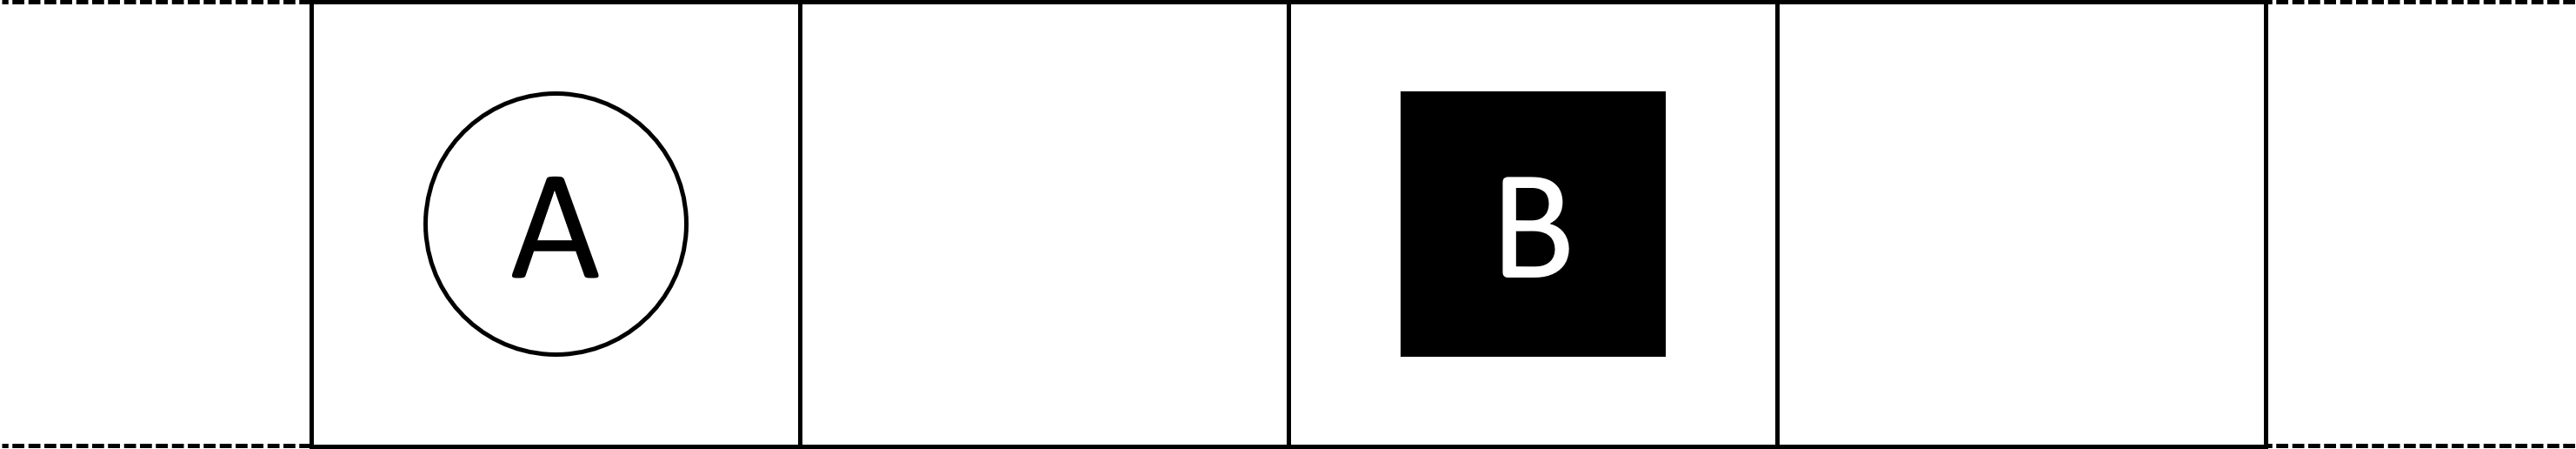
\includegraphics[width=\textwidth]{5BeyondSBDRL/Old/Images/Movable_block_world_states/w6.png}
    \caption{$w_{6}$}
  \end{subfigure}%
  \hfill
  \begin{subfigure}{0.48\textwidth}
    \centering
    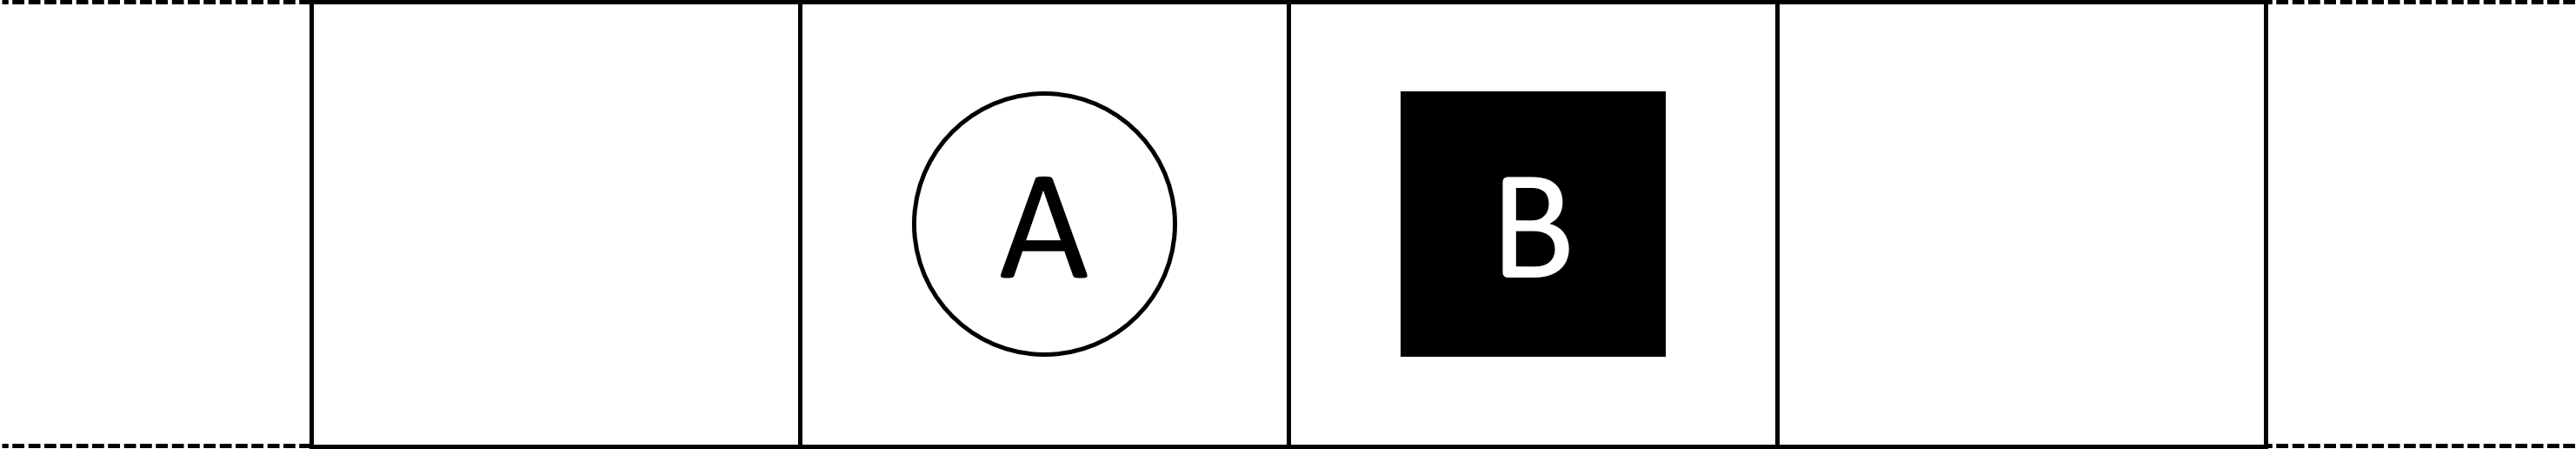
\includegraphics[width=\textwidth]{5BeyondSBDRL/Old/Images/Movable_block_world_states/w7.png}
    \caption{$w_{7}$}
  \end{subfigure}%
  \vspace{0.5cm}
  \begin{subfigure}{0.48\textwidth}
    \centering
    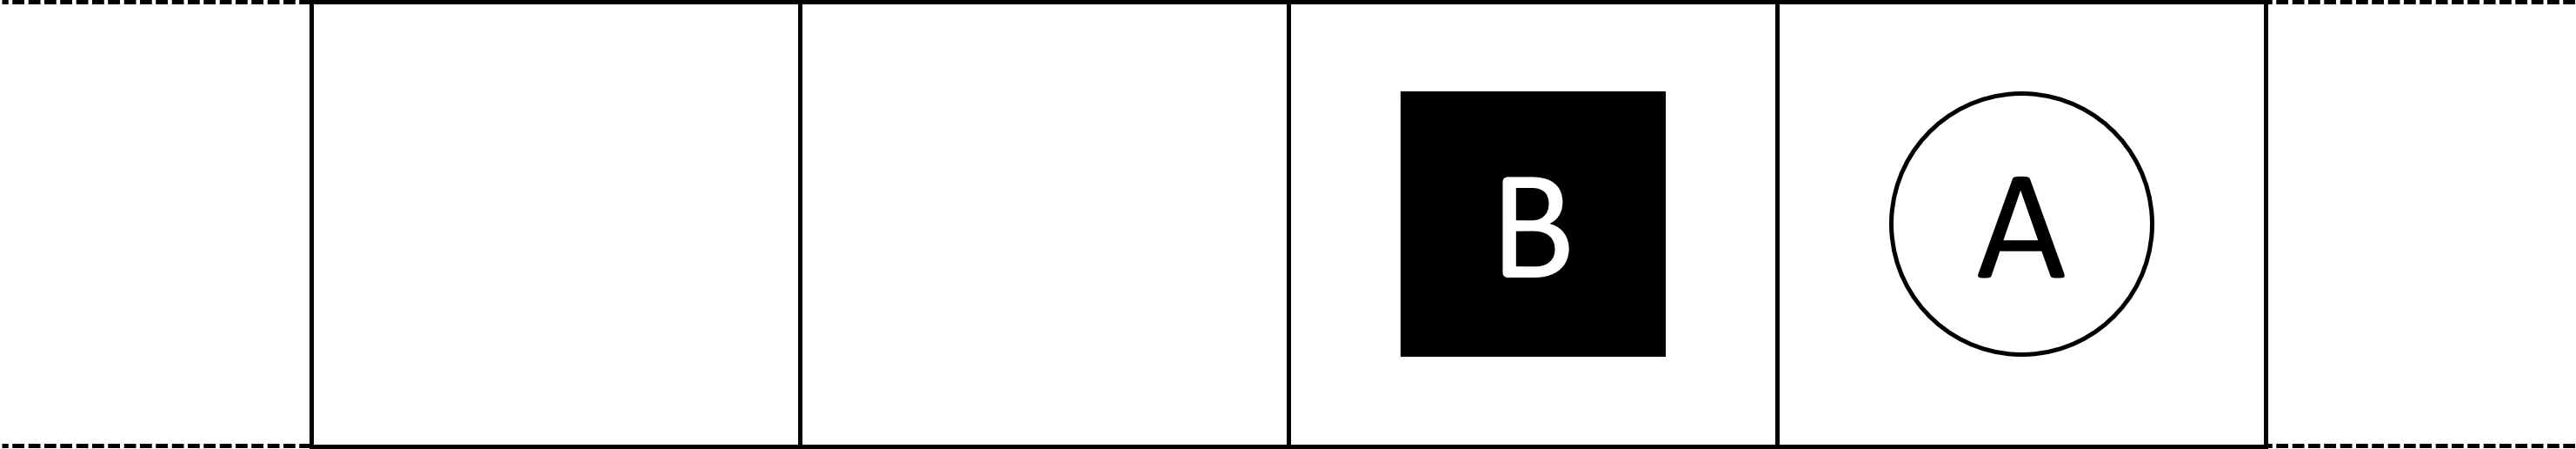
\includegraphics[width=\textwidth]{5BeyondSBDRL/Old/Images/Movable_block_world_states/w8.png}
    \caption{$w_{8}$}
  \end{subfigure}%
  \hfill
  \begin{subfigure}{0.48\textwidth}
    \centering
    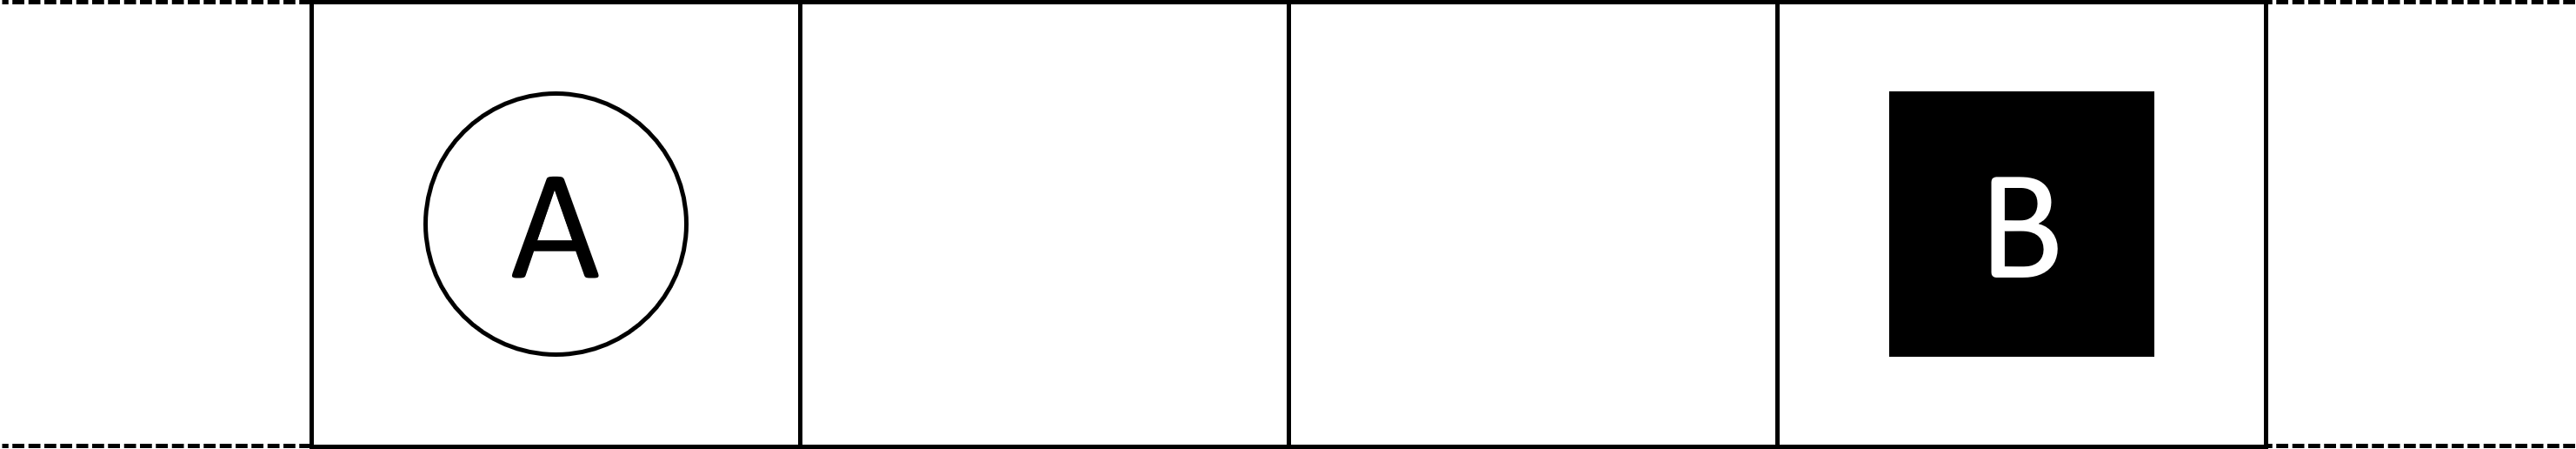
\includegraphics[width=\textwidth]{5BeyondSBDRL/Old/Images/Movable_block_world_states/w9.png}
    \caption{$w_{9}$}
  \end{subfigure}%
    \vspace{0.5cm}
  \begin{subfigure}{0.48\textwidth}
    \centering
    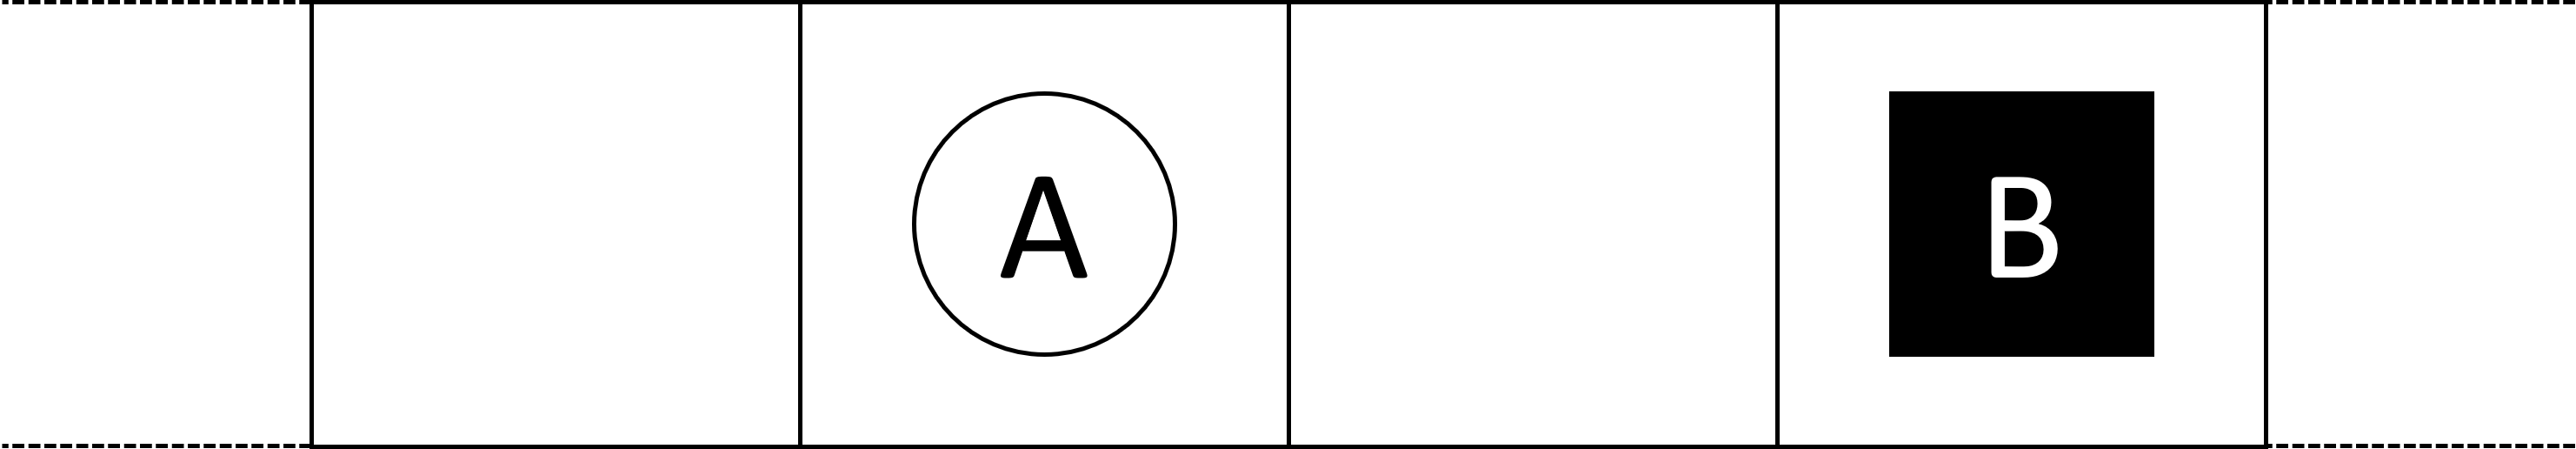
\includegraphics[width=\textwidth]{5BeyondSBDRL/Old/Images/Movable_block_world_states/w10.png}
    \caption{$w_{10}$}
  \end{subfigure}%
  \hfill
  \begin{subfigure}{0.48\textwidth}
    \centering
    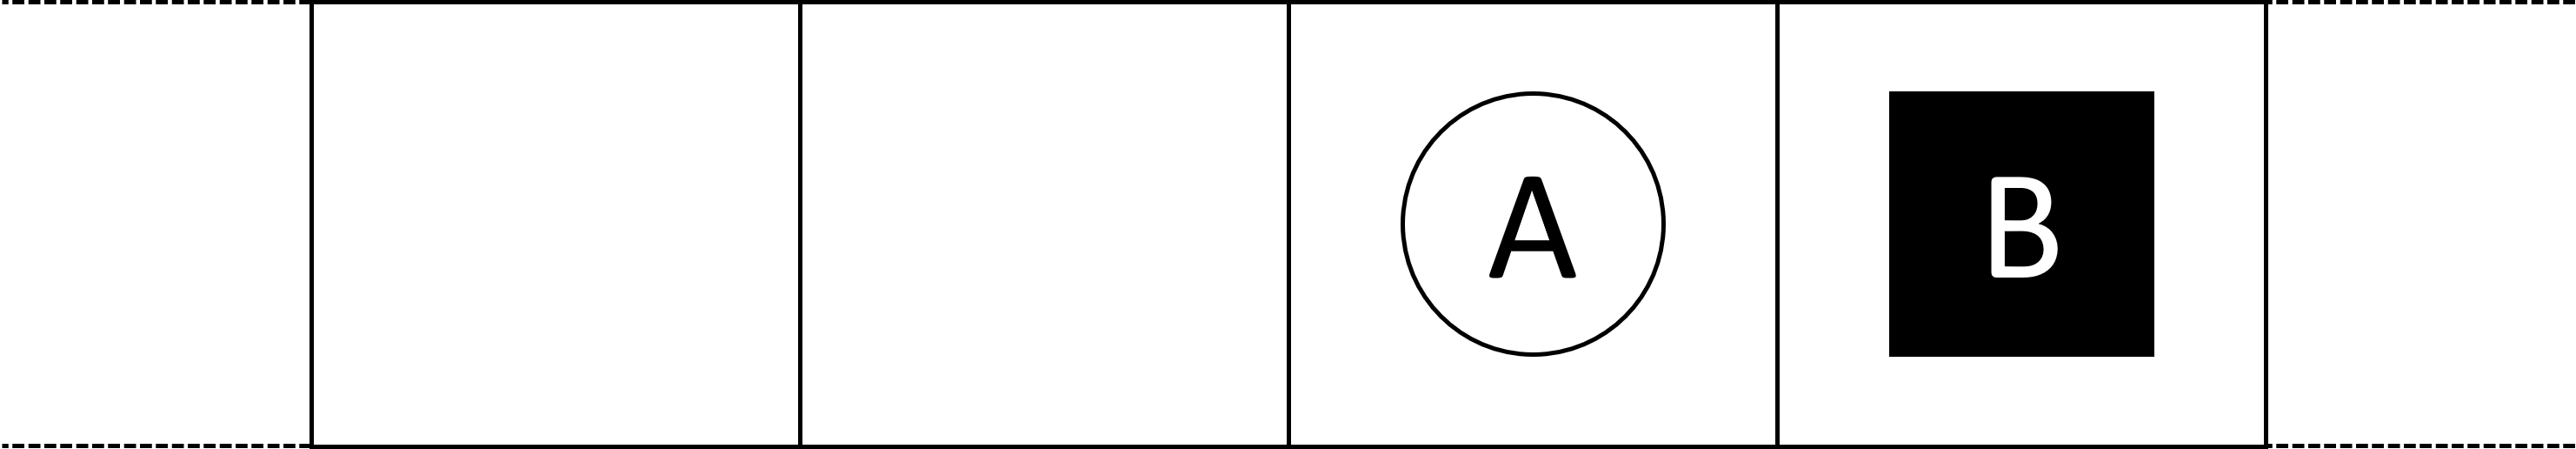
\includegraphics[width=\textwidth]{5BeyondSBDRL/Old/Images/Movable_block_world_states/w11.png}
    \caption{$w_{11}$}
  \end{subfigure}%
  \caption{World states of a world containing an agent and a movable block.}
  \label{fig:movable_block_world_states}
\end{figure}

\begin{table}[H]
    \centering
    \begin{tabular}{c|c c c c c}
                &  $1$      & $L$      & $R$\\
         \hline
        $w_{0}$ & $w_{0}$   & $w_{9}$   & $w_{1}$\\
        $w_{1}$ & $w_{1}$   & $w_{0}$   & $w_{2}$\\
        $w_{2}$ & $w_{2}$   & $w_{1}$   & $w_{3}$\\
        $w_{3}$ & $w_{3}$   & $w_{5}$   & $w_{7}$\\
        $w_{4}$ & $w_{4}$   & $w_{0}$   & $w_{5}$\\
        $w_{5}$ & $w_{5}$   & $w_{4}$   & $w_{3}$\\
        $w_{6}$ & $w_{6}$   & $w_{8}$   & $w_{7}$\\
        $w_{7}$ & $w_{7}$   & $w_{6}$   & $w_{11}$\\
        $w_{8}$ & $w_{8}$   & $w_{4}$   & $w_{6}$\\
        $w_{9}$ & $w_{9}$   & $w_{8}$   & $w_{10}$\\
        $w_{10}$ & $w_{10}$ & $w_{9}$   & $w_{11}$\\
        $w_{11}$ & $w_{11}$ & $w_{10}$  & $w_{2}$\\
    \end{tabular}
    \caption{
    Each entry in this table shows the outcome state of the agent performing the action given in the column label when in the world state given by the row label.
    }
    \label{tab:4x1-gridworld-minimum-transitions-moveable-block}
\end{table}

\begin{figure}[H]
    \centering
    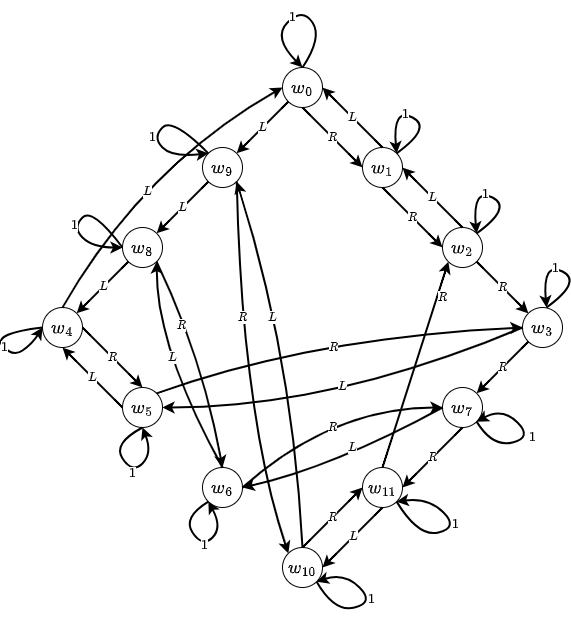
\includegraphics[width=0.7\linewidth]{5BeyondSBDRL/Old/Images/fig-4x1-block-min-actions-wall.png}
    \caption{
    A transition diagram of the labelled transitions in Table \ref{tab:4x1-gridworld-minimum-transitions-moveable-block}.
    }
    \label{fig:4x1-block-min-actions-wall}
\end{figure}

The action Cayley table for $\mathscr{W}_{block}$ contains 17 elements.
As shown by Table \ref{tab:block-world-properties}, $A/\sim$ is a monoid.

\begin{table}[H]
    \centering
    \begin{tabular}{c|c}
        \textbf{Property}   & \textbf{Present?} \\
        \hline
        Totality            & Y\\
        Identity            & Y\\
        Inverse             & N\\
        Associative         & Y\\
        Commutative         & N
    \end{tabular}
    \caption{Properties of the $A/\sim$ algebra.}
    \label{tab:block-world-properties}
\end{table}

\begin{remark}
    Adding a wall or a moveable block breaks the symmetry of the original $2 \times 2$ cyclical world $\mathscr{W}_{c}$; this manifests as the action algebra of the world being much more complex.
\end{remark}

%%%%%%%%%%%%%%%%%%%%%%%%%%%%%%%%%%%%%%%%%%%%%%%%%%%%%%%%%%%%%%
\subsection{Example 3: irreversible inhomogeneous actions}\label{sec:identity irreversible inhomogeneous actions}

This example explores the transition algebras of worlds that are action-inhomogeneous and contain irreversible actions.

Consider a world $\mathscr{W}_{consumable}$ with movement along a single 1D cyclical axis with a single consumable.
Let this world also contain an agent that can move left, right or consume the consumable if the agent is in the same place as the consumable.

\begin{figure}[H]
  \centering
  \begin{subfigure}{0.48\textwidth}
    \centering
    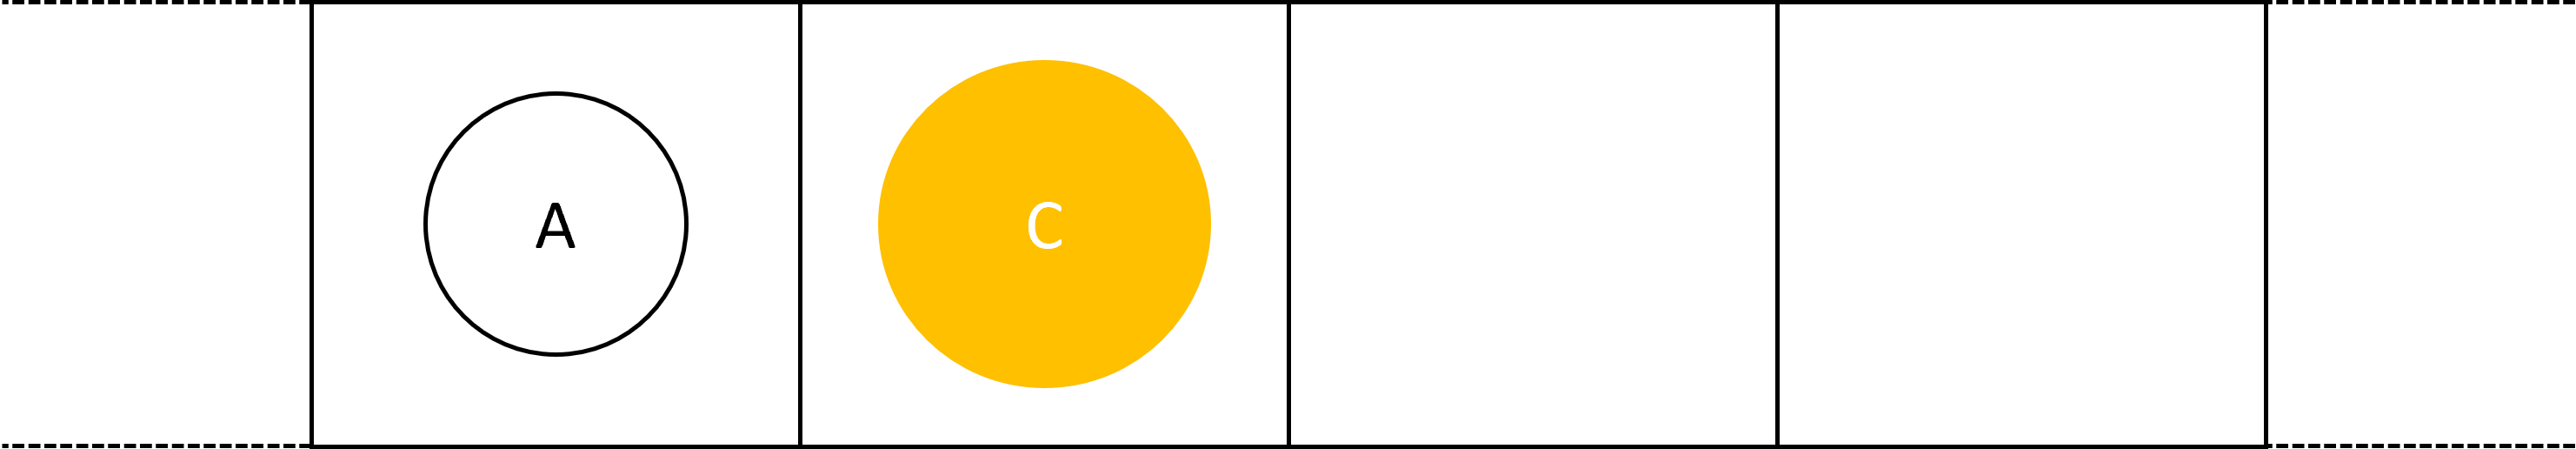
\includegraphics[width=\textwidth]{5BeyondSBDRL/Old/Images/Consumable_world_states/w0.png}
    \caption{$w_{0}$}
    \label{fig:w0}
  \end{subfigure}%
  \hfill
  \begin{subfigure}{0.48\textwidth}
    \centering
    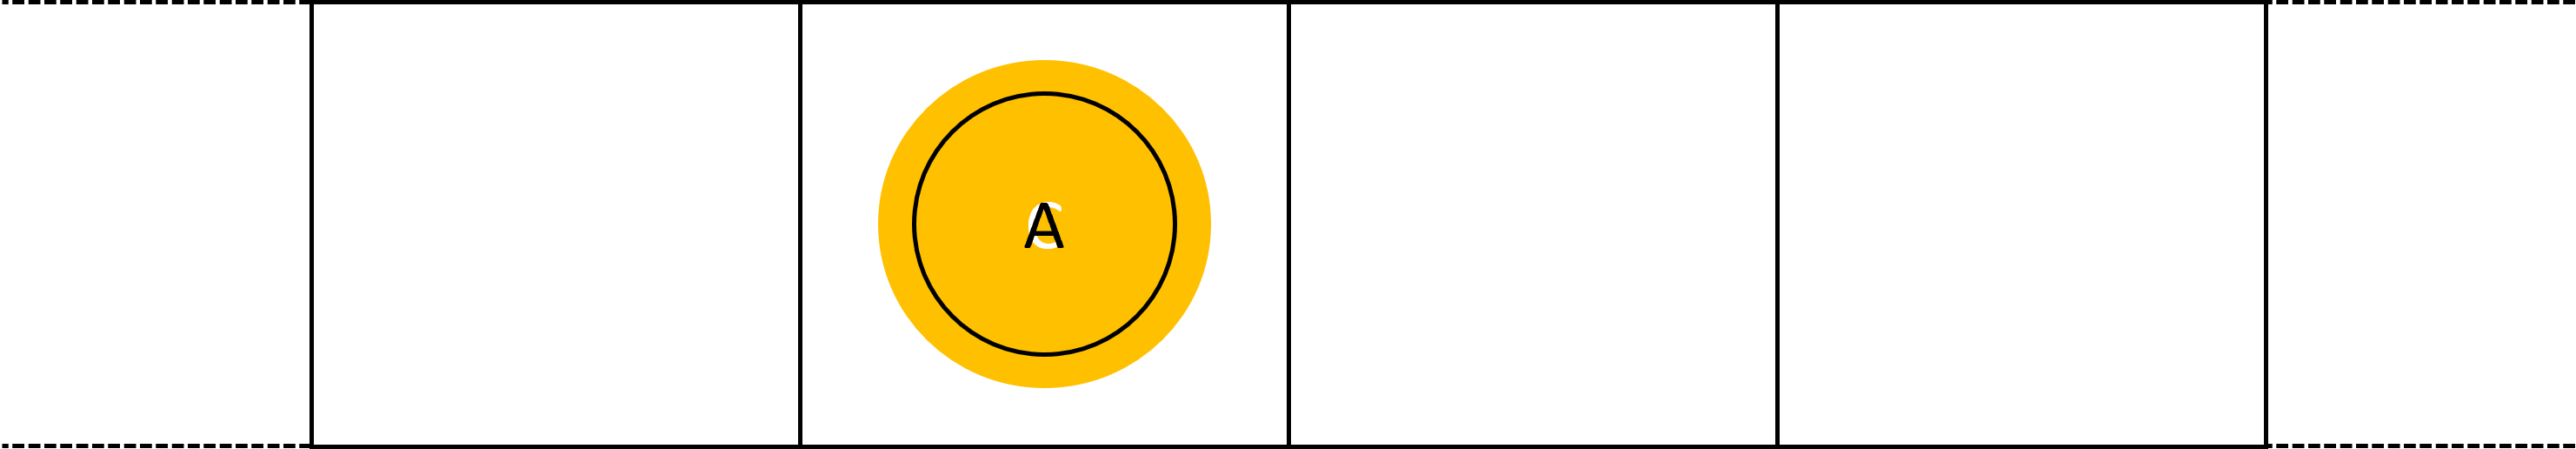
\includegraphics[width=\textwidth]{5BeyondSBDRL/Old/Images/Consumable_world_states/w1.png}
    \caption{$w_{1}$}
    \label{fig:w1}
  \end{subfigure}%
  \vspace{0.5cm}
  \begin{subfigure}{0.48\textwidth}
    \centering
    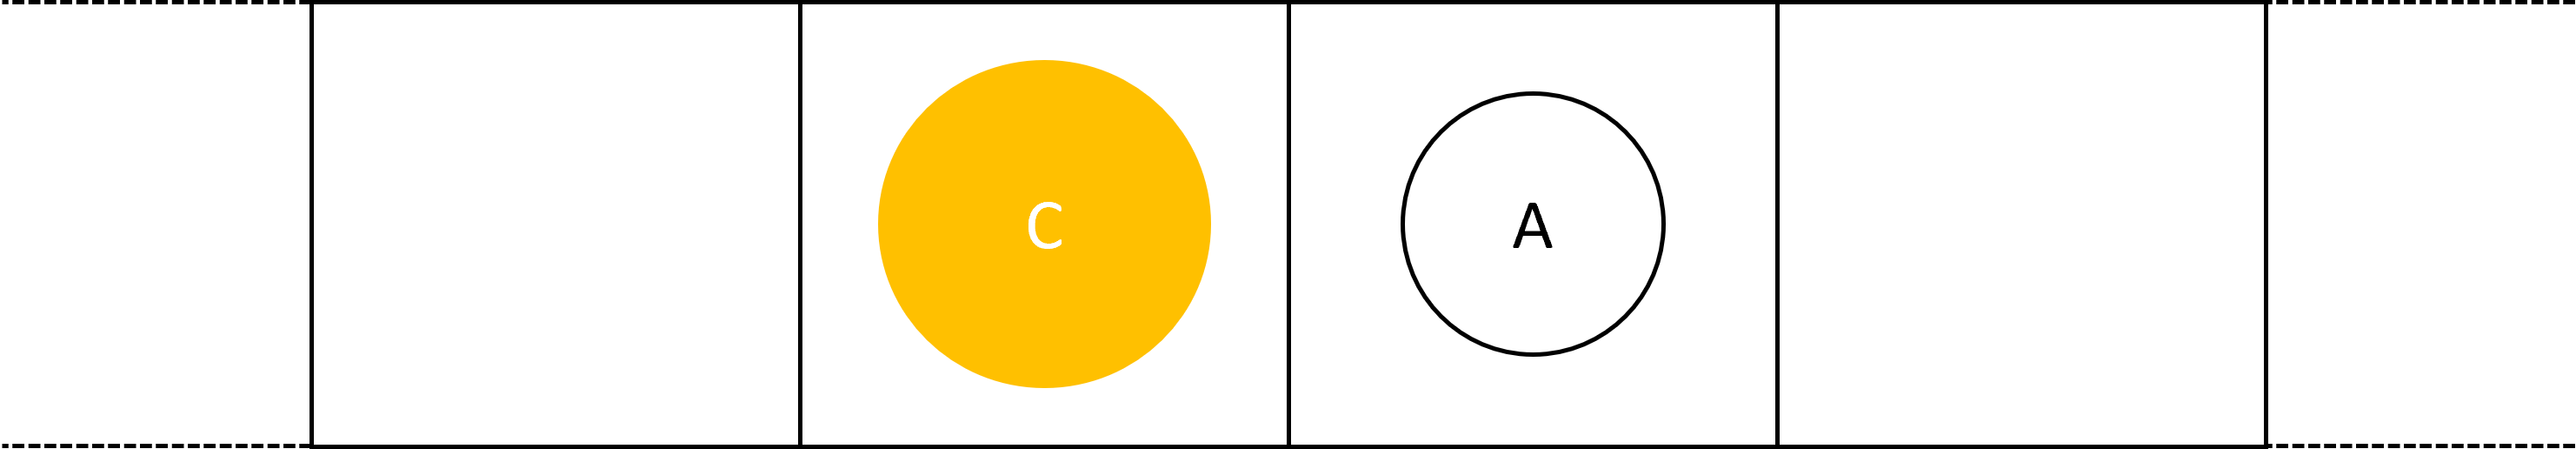
\includegraphics[width=\textwidth]{5BeyondSBDRL/Old/Images/Consumable_world_states/w2.png}
    \caption{$w_{2}$}
    \label{fig:w2}
  \end{subfigure}%
  \hfill
  \begin{subfigure}{0.48\textwidth}
    \centering
    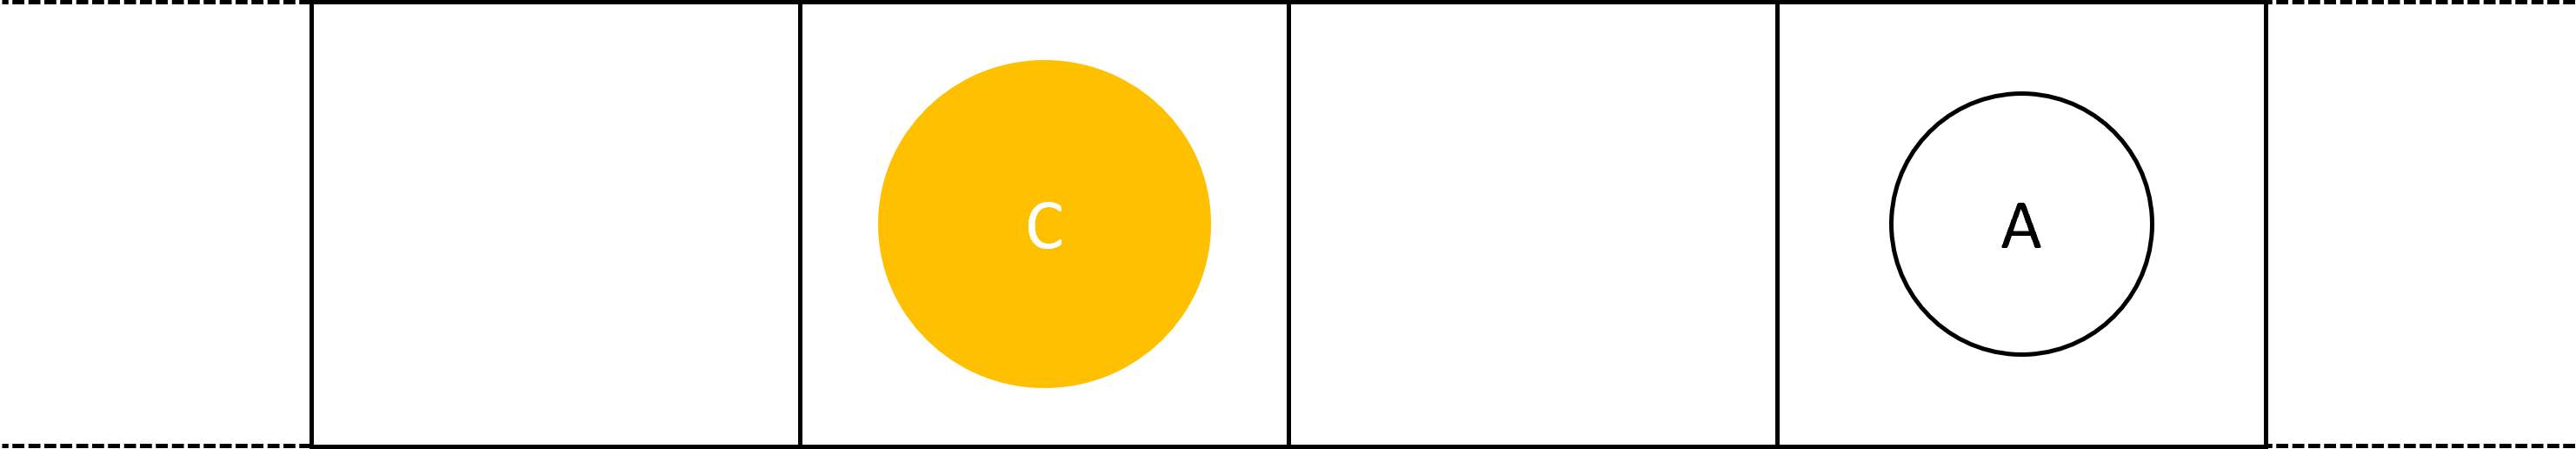
\includegraphics[width=\textwidth]{5BeyondSBDRL/Old/Images/Consumable_world_states/w3.png}
    \caption{$w_{3}$}
    \label{fig:w3}
  \end{subfigure}%
  \vspace{0.5cm}
  \begin{subfigure}{0.48\textwidth}
    \centering
    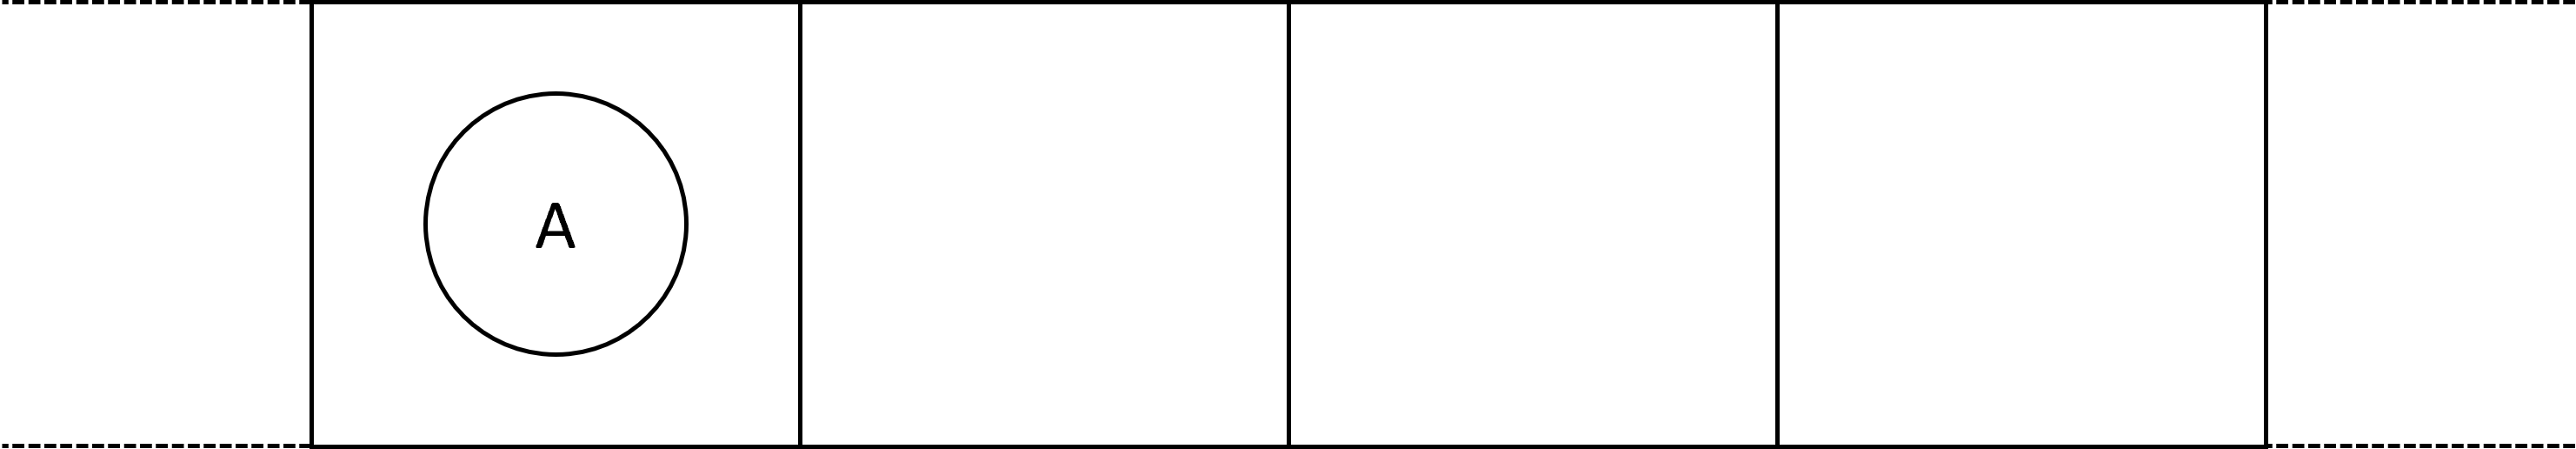
\includegraphics[width=\textwidth]{5BeyondSBDRL/Old/Images/Consumable_world_states/w4.png}
    \caption{$w_{4}$}
    \label{fig:w4}
  \end{subfigure}%
  \hfill
  \begin{subfigure}{0.48\textwidth}
    \centering
    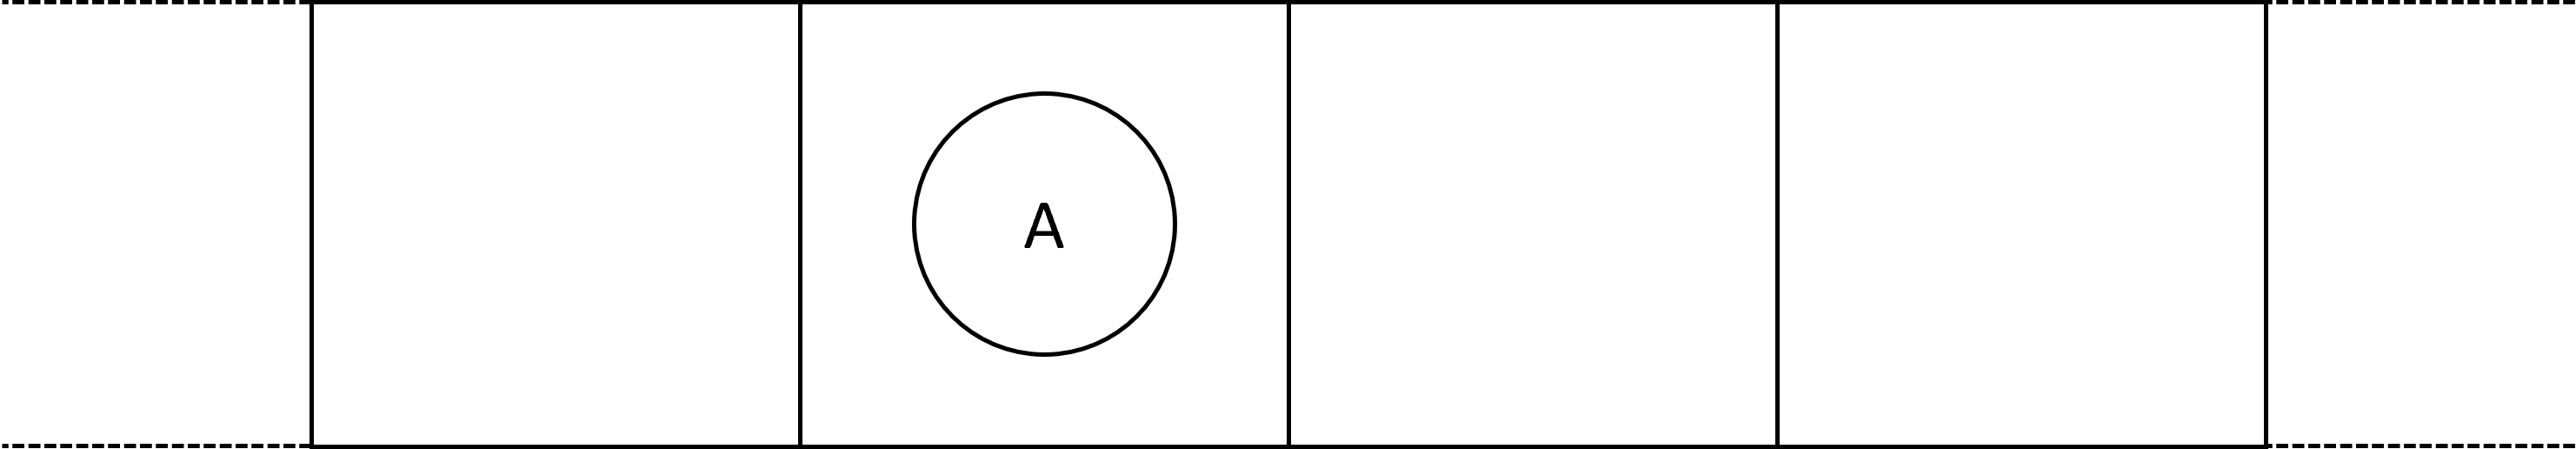
\includegraphics[width=\textwidth]{5BeyondSBDRL/Old/Images/Consumable_world_states/w5.png}
    \caption{$w_{5}$}
    \label{fig:w5}
  \end{subfigure}%
  \vspace{0.5cm}
  \begin{subfigure}{0.48\textwidth}
    \centering
    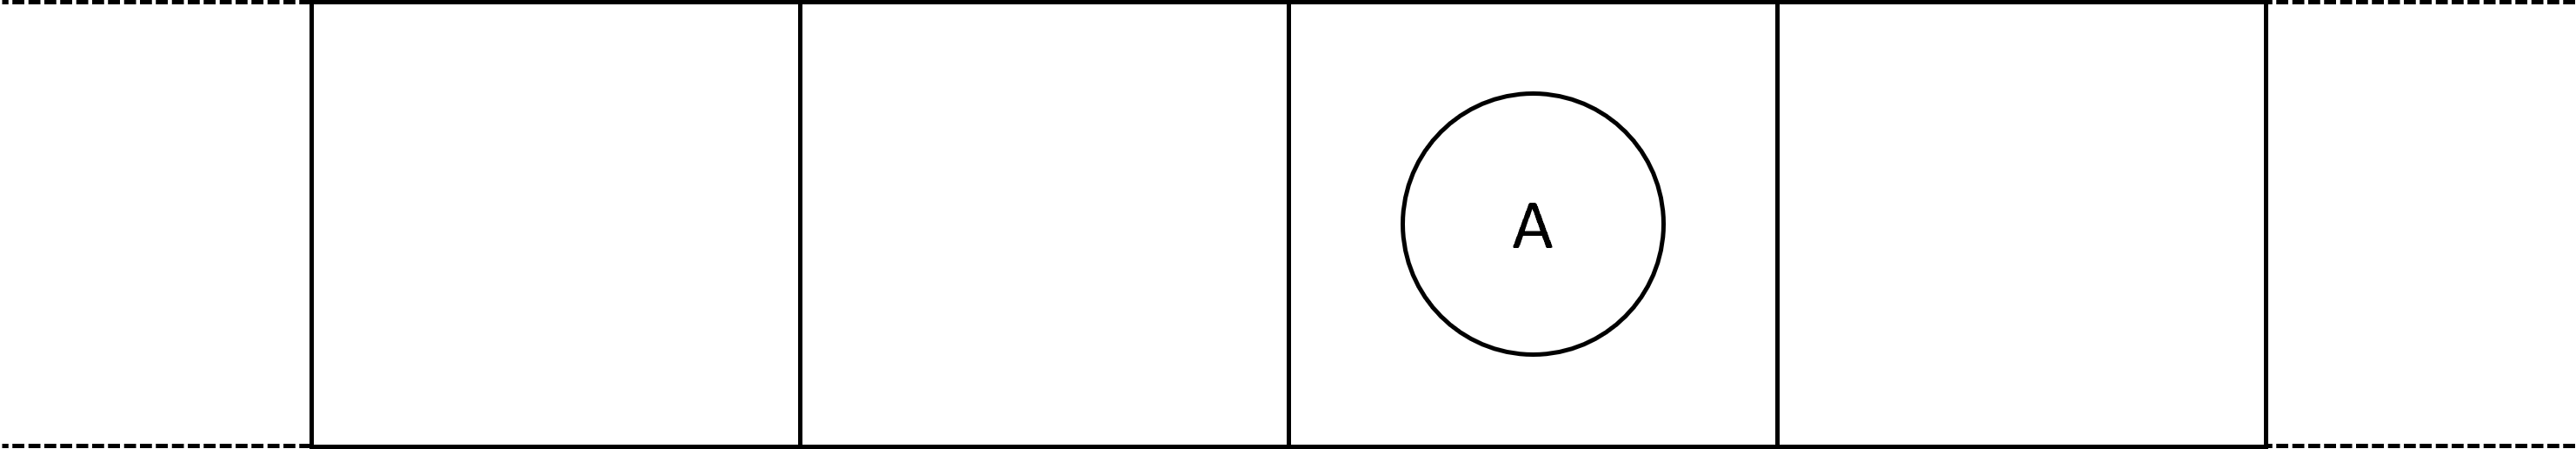
\includegraphics[width=\textwidth]{5BeyondSBDRL/Old/Images/Consumable_world_states/w6.png}
    \caption{$w_{6}$}
    \label{fig:w6}
  \end{subfigure}%
  \hfill
  \begin{subfigure}{0.48\textwidth}
    \centering
    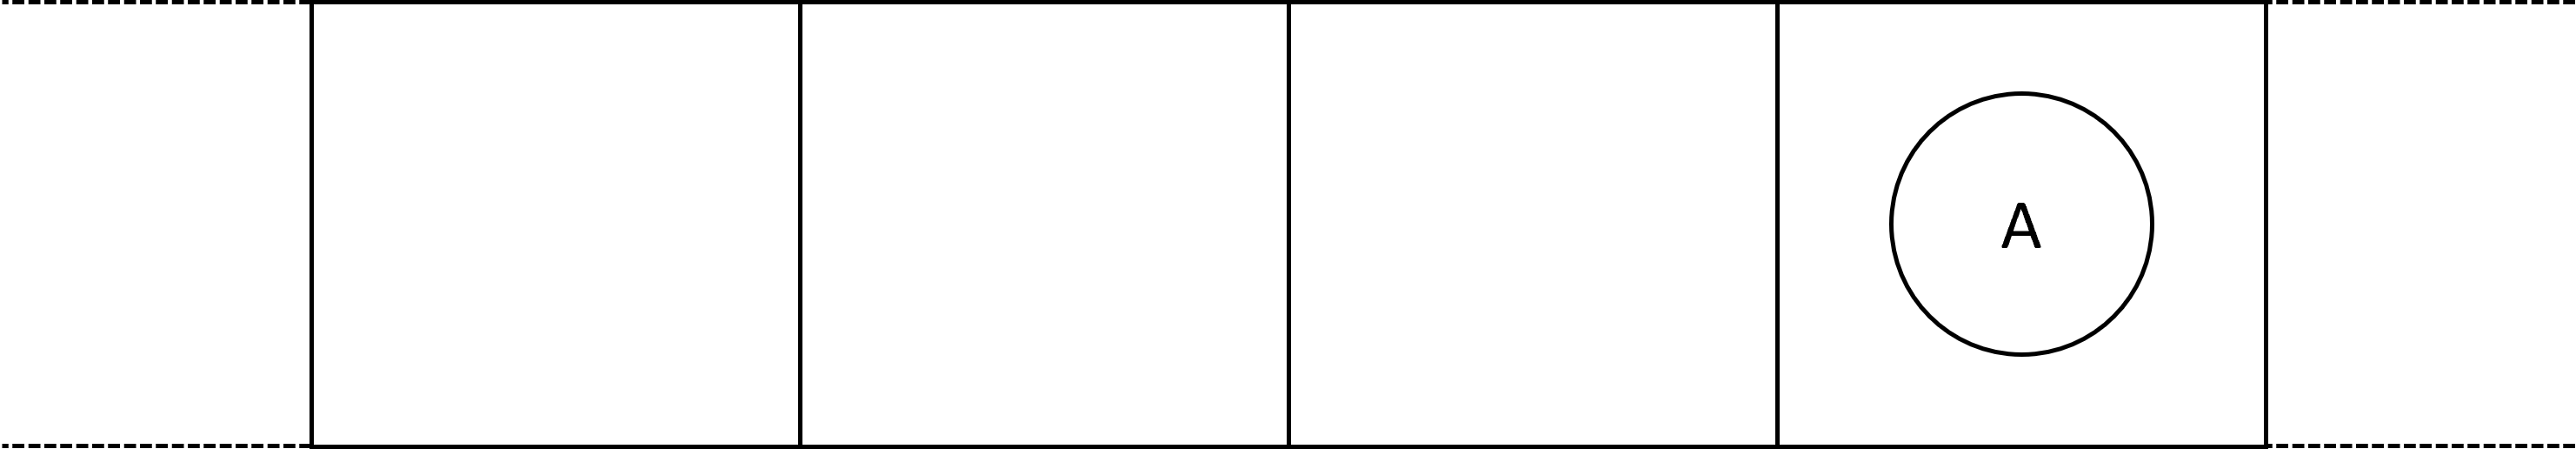
\includegraphics[width=\textwidth]{5BeyondSBDRL/Old/Images/Consumable_world_states/w7.png}
    \caption{$w_{7}$}
    \label{fig:w7}
  \end{subfigure}%
  
  \caption{World states of a world containing an agent and a consumable.}
  \label{fig:consumable_world_states}
\end{figure}

There is not a consumable in every state, therefore if the agent performs the consume action in any state except $w_{1}$ then the effect will be the same as if the agent had performed the no-op action $1 \in A/\sim$ (see Figure \ref{fig:min-action-net-world-with-consumable-identity}).

\begin{figure}[H]
    \centering
    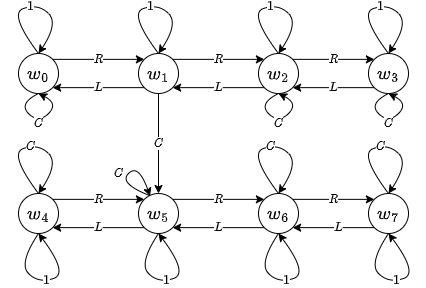
\includegraphics[width=0.7\linewidth]{5BeyondSBDRL/Old/Images/fig-min-action-net-world-with-consumable-identity.png}
    \caption{
   Minimum action network for world $\mathscr{W}_{consumable}$.
    }
    \label{fig:min-action-net-world-with-consumable-identity}
\end{figure}

The action Cayley table for world $\mathscr{W}_{consumable}$ with restricted actions treated as identity actions contains 64 elements.
As shown in Table \ref{tab:identity-consumable-properties}, $A/\sim$ is a monoid.

\begin{table}[H]
    \centering
    \begin{tabular}{c|c}
        \textbf{Property}   & \textbf{Present?} \\
        \hline
        Totality            & Y\\
        Identity            & Y\\
        Inverse             & N\\
        Associative         & Y\\
        Commutative         & N
    \end{tabular}
    \caption{Properties of the $A/\sim$ algebra.}
    \label{tab:identity-consumable-properties}
\end{table}

\begin{remark}
    Considering this example, we note that the irreversible action moves from one `reversible plane' to another.
    Perhaps we can treat an irreversible action as having a `reversible action affecting part' and a `world affecting part'; in this example, the reversible action affecting part would be the identity action since the reversible action network is unchanged by the irreversible action.
\end{remark}

%%%%%%%%%%%%%%%%%%%%%%%%%%%%%%%%%%%%%%%%%%%%%%%%%%%%%%%%%%%%%%%%%%%%%%%%%%%%%%
\section{Worlds without inverse actions or unrestricted actions}\label{sec:Worlds without inverse actions or unrestricted actions}

In this section, we consider worlds that do not necessarily satisfy world condition ref[wldcon:inverse-actions] or world condition ref[wldcon:unrestricted-actions].

\begin{proposition}\label{prp:all_worlds_give_small_category_action}
    Consider a world $\mathscr{W}$ with a set $W$ of world states and containing an agent with a set $A$ of actions.
    $*: (A/\sim) \times W \to W'$, where $W' \subseteq W$, is the action of a small category $A/\sim$ on $W$.
\end{proposition}
\begin{proof}
    (1) Associativity of $A/\sim$ is given by proposition ref[prp:Asim-associative].
    (2) Identity element of $A/\sim$ is given by proposition ref[prp:Asim-identity].
    Since $A/\sim$ satisfies properties (1) and (2), $A/\sim$ is a small category.
    Therefore $*$ is the action of a small category.
\end{proof}

\begin{remark}
    We can consider two equivalent perspectives of $*$:
    \begin{enumerate}
        \item $A/\sim$ is a small category and $*$ is a full action of $A/\sim$ on $W$.
        \item $A/\sim$ is a monoid and $*$ is a partial action of $A/\sim$ on $W$.
    \end{enumerate}
\end{remark}

%%%%%%%%%%%%%%%%%%%%%%%%%%%%%%%%%%%%%%
\subsection{Example 1: reversible action-inhomogeneous world}\label{sec:masked reversible action-inhomogeneous world}

We once again consider the world $\mathscr{W}_{wall}$ (see Figure \ref{fig:2x2-cyclical-grid-world-wall-states} for world states); however, now instead of treating restricted actions like the identity action, we \textit{mask} the restricted actions.
Masking restricted actions involves not allowing the agent to perform the restricted actions - the restricted actions are hidden (masked) from the agent - and so, mathematically, we treat the restricted actions as \textit{undefined}; for example, if $\mathscr{W}_{wall}$ is in state $w_{0}$, then the agent cannot perform the $R$ action because $R * w_{0}$ is undefined.





The action Cayley table for $\mathscr{W}_{wall}$ with the masked treatment of the walls contains 59 elements.
As shown in Table \ref{tab:masked-walls}, $A/\sim$ is a small category.

\begin{table}[H]
    \centering
    \begin{tabular}{c|c}
        \textbf{Property}   & \textbf{Present?} \\
        \hline
        Totality            & N\\
        Identity            & Y\\
        Inverse             & N\\
        Associative         & Y\\
        Commutative         & N
    \end{tabular}
    \caption{Properties of the $A/\sim$ algebra.}
    \label{tab:masked-walls}
\end{table}

%%%%%%%%%%%%%%%%%%%%%%%%%%%%%%%%%%%%%%
\subsection{Example 2: irreversible action-inhomogeneous world}\label{sec:masked irreversible action-inhomogeneous world}

We will now apply the masking treatment of restricted actions to the world $\mathscr{W}_{consumable}$ (see Figure \ref{fig:consumable_world_states} for world states); for example, if $\mathscr{W}_{consumable}$ is not in state $w_{1}$ then the consume action is undefined.

\begin{figure}[H]
    \centering
    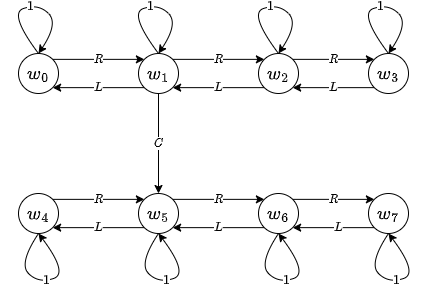
\includegraphics[scale=0.5]{5BeyondSBDRL/Old/Images/fig-min-action-net-world-with-consumable-masked.png}
    \caption{Minimum action network for world containing an agent and a consumable.}
    \label{fig-min-action-net-world-with-consumable-masked}
\end{figure}

The action Cayley table for $\mathscr{W}_{consumable}$ with the masked treatment of the walls contains 20 elements.
As shown in Table \ref{tab:masked-consumable-properties}, $A/\sim$ is a small category.

\begin{table}[H]
    \centering
    \begin{tabular}{c|c}
        \textbf{Property}   & \textbf{Present?} \\
        \hline
        Totality            & N\\
        Identity            & Y\\
        Inverse             & N\\
        Associative         & Y\\
        Commutative         & N
    \end{tabular}
    \caption{Properties of the $A/\sim$ algebra.}
    \label{tab:masked-consumable-properties}
\end{table}








-------------

\begin{remark}
    \draftnote{blue}{Consider}{
    Make this about state Cayley tables ?
    }
    For any world, once the agent has the action Cayley table for any initial world state it can produce the action Cayley table for any other initial world state by applying an action that transitions from the old initial world state to the new initial world state to every element of the action Cayley table.
\end{remark}

\draftnote{blue}{To do}{
Can we prove something about this?
e.g., 
}
We have also demonstrated that neither the identity treatment nor the masked treatment produces the more simple algebra in every world.
For $\mathscr{W}_{wall}$, the identity treatment contains fewer elements than the masked treatment (26 elements vs 59 elements), while for $\mathscr{W}_{consumable}$ the masked treatment contains fewer elements than the identity treatment (20 elements vs 64 elements).



